%%%%%%%%%%%%%%%%%%%%%%%%%%%%%%%%%%%%%%%%%%%%%%%%%%%%%%%%%%%%%%%%%%%%%%%%%%%%%%%
\section{Using MGXS in Multi-Group Eigenvalue Calculations}
\label{sec:evaluation}
%%%%%%%%%%%%%%%%%%%%%%%%%%%%%%%%%%%%%%%%%%%%%%%%%%%%%%%%%%%%%%%%%%%%%%%%%%%%%%%

Need to


%%%%%%%%%%%%%%%%%%%%%%%%%%%%%%%%%%%%%%%%%%%%%
\subsection{Benchmarks and Reference Results}
\label{subsec:benchmarks}

Two benchmarks were derived from the Benchmark for Evaluation And Validation of Reactor Simulations (BEAVRS) PWR model~\cite{horelik2013beavrs} to validate the \texttt{openmc.mgxs} module. Both benchmarks included a heterogeneous composition of 1.6\% and 3.1\% enriched UO$_2$ fuel, borated water, zircaloy, helium, air, borosilicate glass and stainless steel. The isotopic compositions of the materials, and the geometric configurations of each pin type were identical to those given in the BEAVRS specifications and will not be reproduced here. The continuous energy cross sections were from the ENDF/B-VII.1 library~\cite{mcnpx2003manual} evaluated at 600K for hot power conditions.

The first benchmark was a fuel assembly comprised of 264 pins of 1.6\% enriched fuel, 24 control rod guide tubes (CRGTS) and a single central instrument tube. The assembly was modeled with reflective boundary conditions. The second benchmark was a 2$\times$2 colorset of fuel assemblies surrounded by a water reflector on the bottom and right. The top-left and bottom-right fuel assemblies were identical to the single assembly benchmark. The top-right and bottom-left assemblies were comprised of 264 pins of 3.1\% enriched fuel, 20 CRGTs, four burnable poisons (BPs) and a central instrument tube. The colorset was modeled with reflective boundaries on the top and left and vacuum boundaries on the bottom and right. Although BEAVRS is an axially heterogeneous 3D core model, both benchmarks were fabricated in 2D due to the geometric constraints in OpenMOC. The assembly and colorset are illustrated in \autoref{fig:benchmarks-materials}.

\begin{figure}[h!]
\centering
\begin{subfigure}{0.42\textwidth}
  \centering
  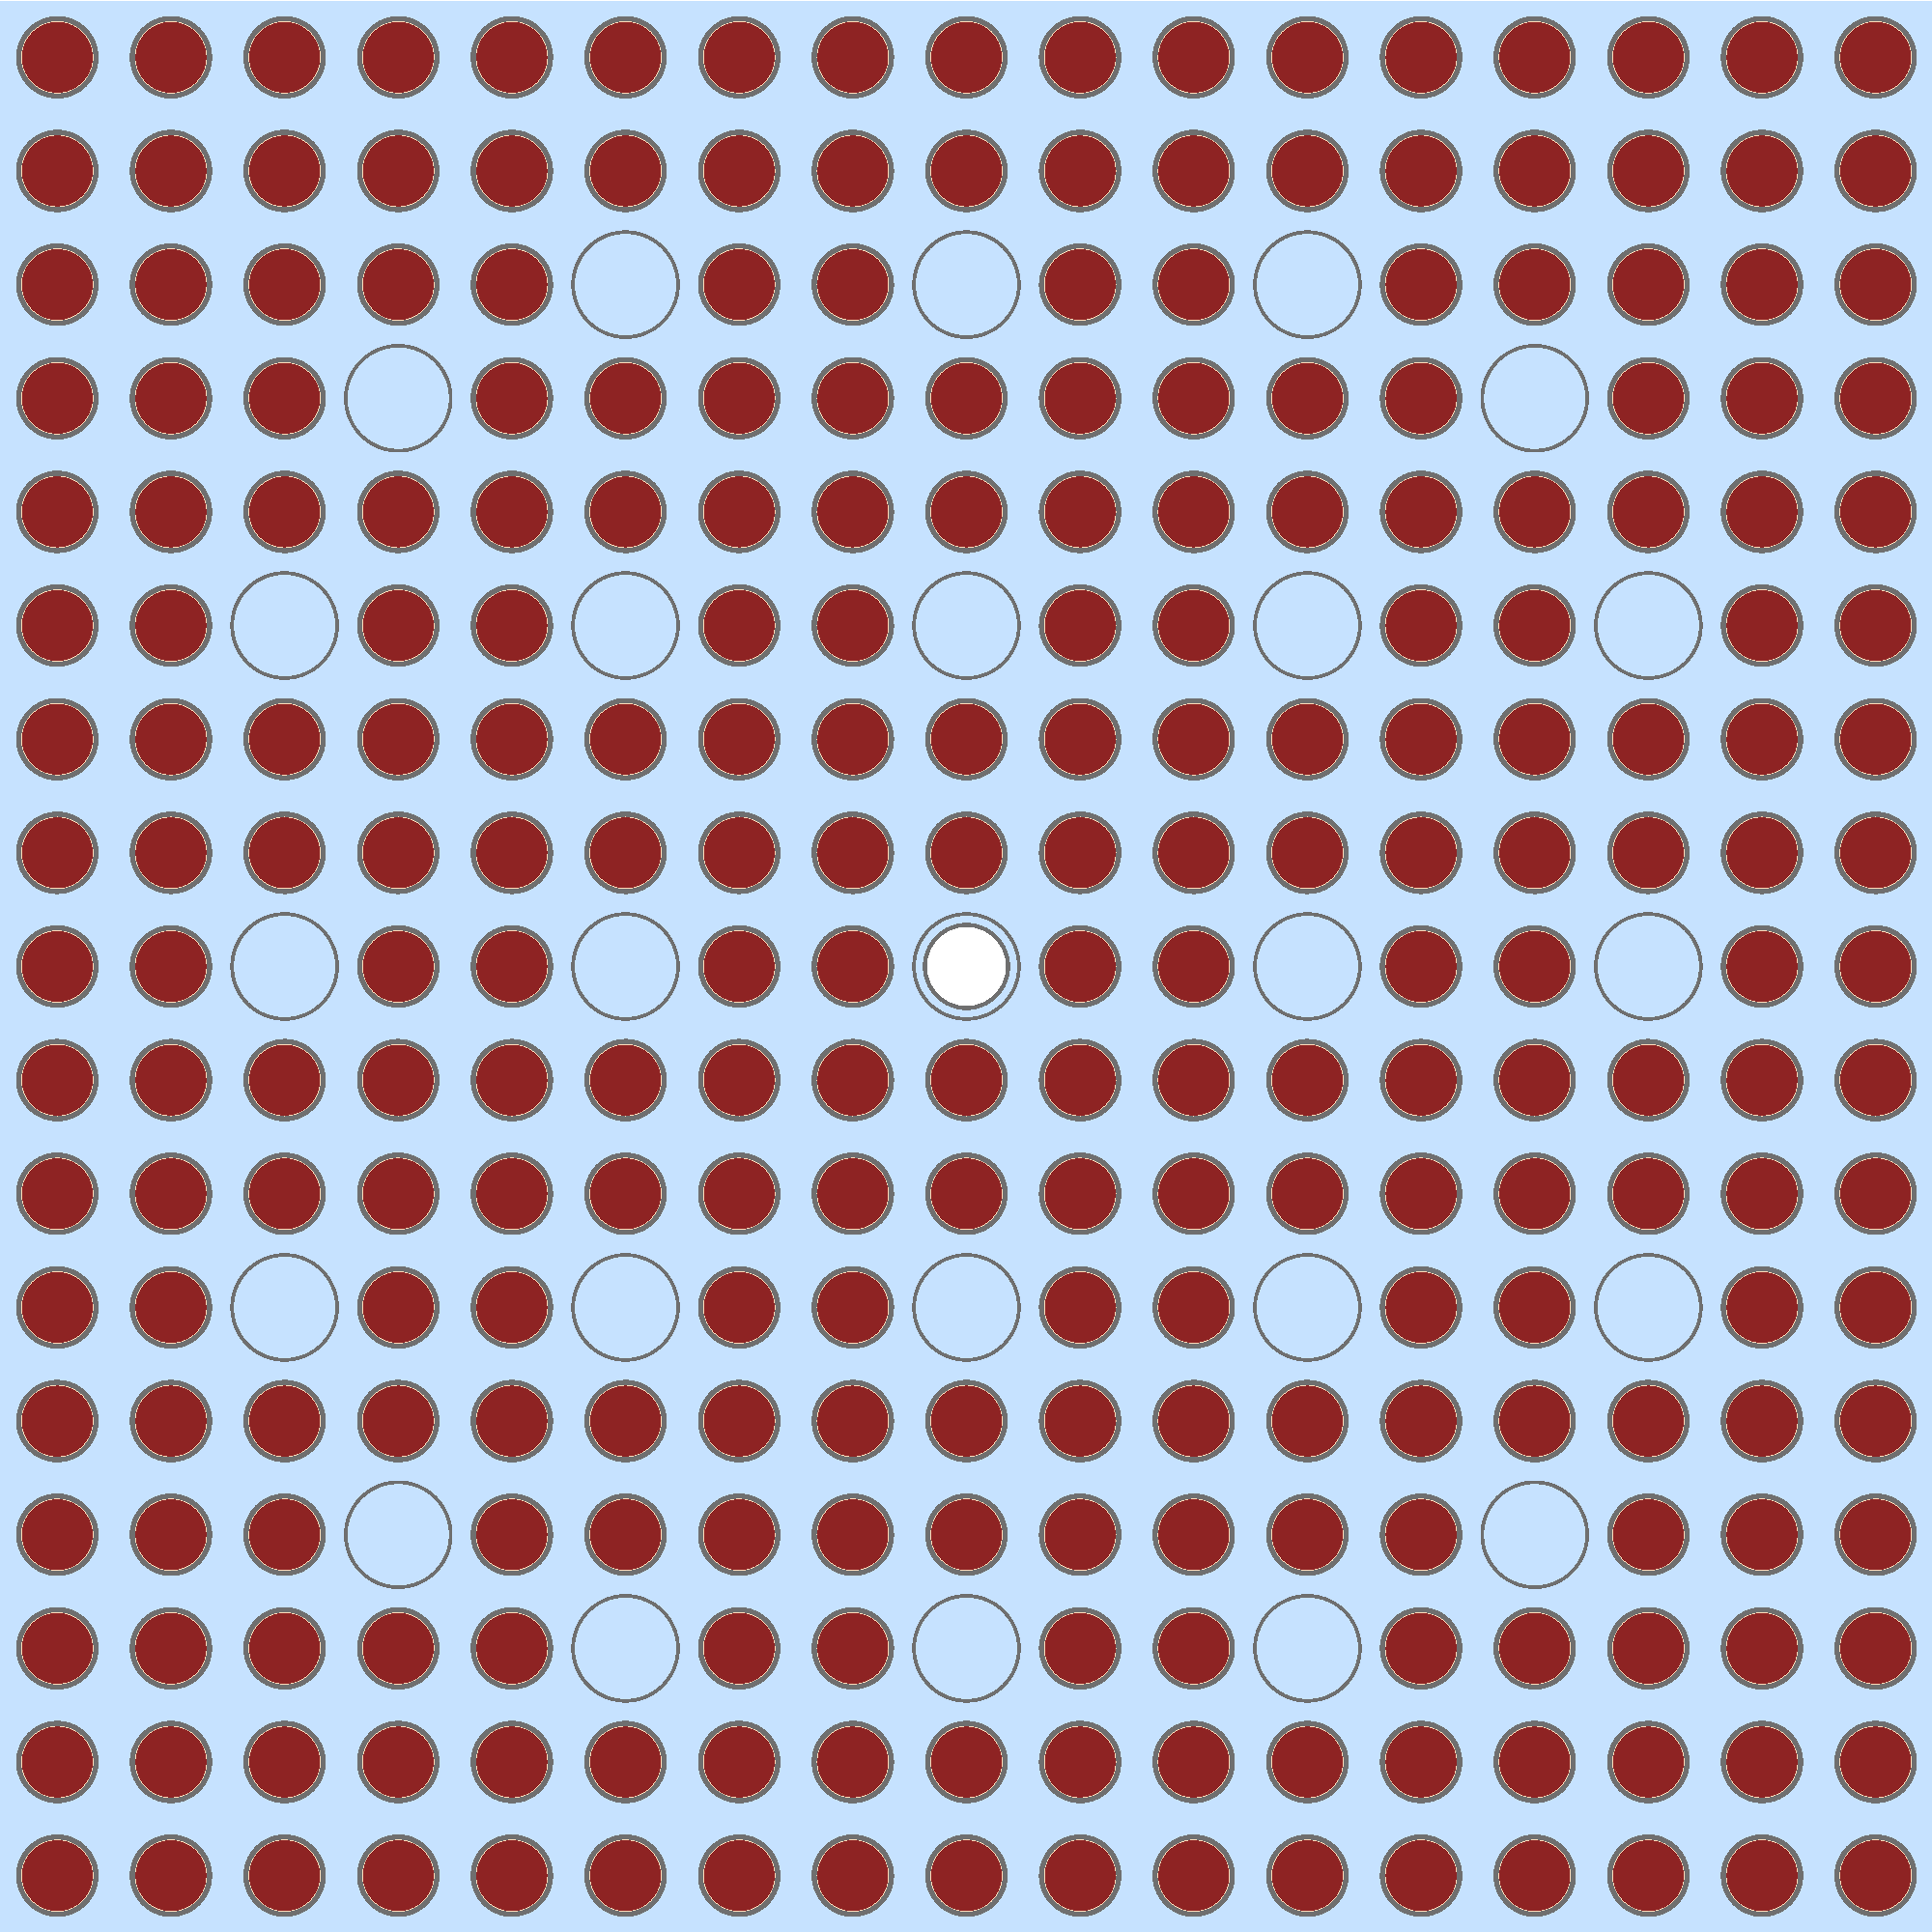
\includegraphics[width=0.8\linewidth]{figures/assembly/geometry}
  \caption{}
  \label{fig:benchmarks}
\end{subfigure}
\begin{subfigure}{0.42\textwidth}
  \centering
  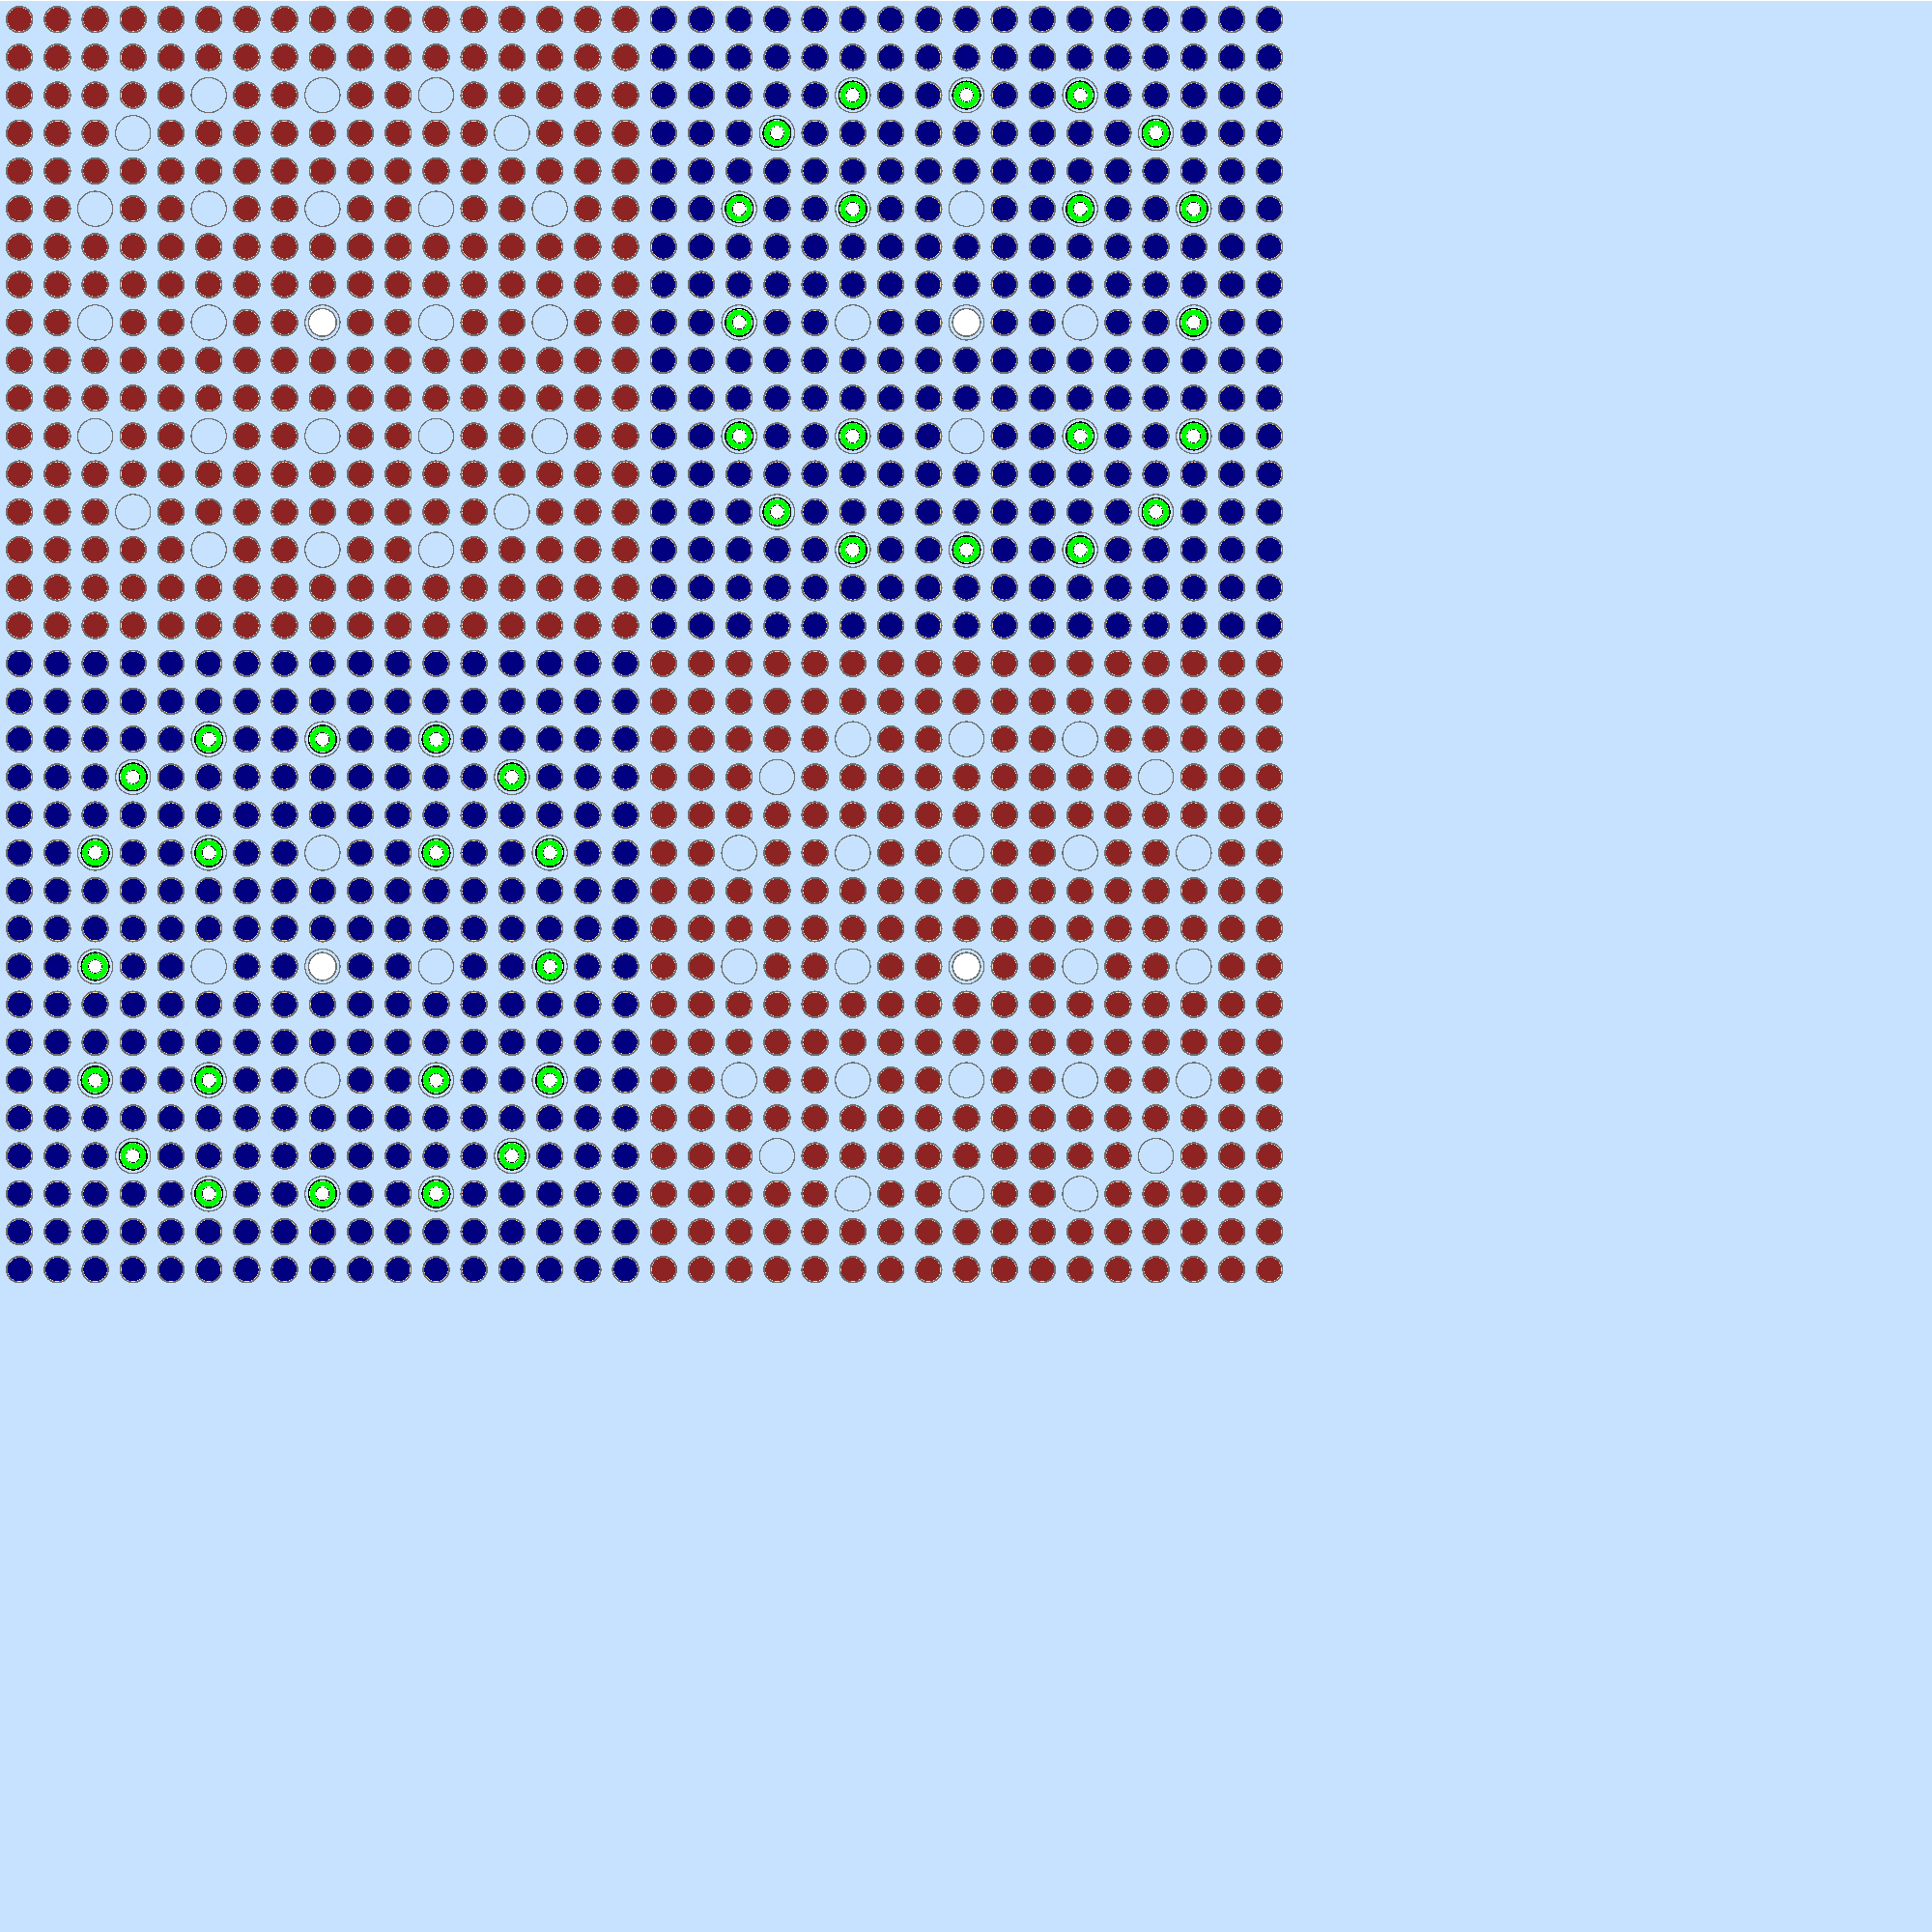
\includegraphics[width=0.8\linewidth]{figures/colorset/geometry}
  \caption{}
  \label{fig:benchmarks-colorset}
\end{subfigure}
\caption{The assembly (a) and colorset (b) benchmark geometries.}
\label{fig:benchmarks-materials}
\end{figure}

OpenMC simulations were used to compute both the MGXS as well as reference eigenvalues and pin-wise fission rates for both benchmarks. The reference solutions were computed with 100 inactive and 900 active batches of 10$^7$ particles histories per batch. The OpenMC reference eigenvalues and their associated 1-sigma uncertainties are reported in \autoref{tab:keff-reference}. Rectilinear, pin-wise tally meshes were used to compute the reference energy-integrated fission rate spatial distributions shown in \autoref{fig:benchmarks-fiss-rates}. The fission rates were normalized to the mean of the non-zero fission rates. The rates in the CRGTs, BPs, and instrument tubes are all zero and are shaded in white. The fission rates have 1-sigma uncertainties of less than 0.08\%.

\begin{table}[h!]
  \centering
  \caption{Reference OpenMC eigenvalues for each benchmark.}
  \label{tab:keff-reference} 
  \begin{tabular}{c c}
  \toprule
  {\bf Assembly} &
  {\bf Colorset} \\
  \midrule
  0.99326 $\pm$ 0.00001 & 0.94574 $\pm$ 0.00001 \\
  \bottomrule
\end{tabular}
\end{table}

\begin{figure*}[h!]
\centering
\begin{subfigure}{0.45\textwidth}
  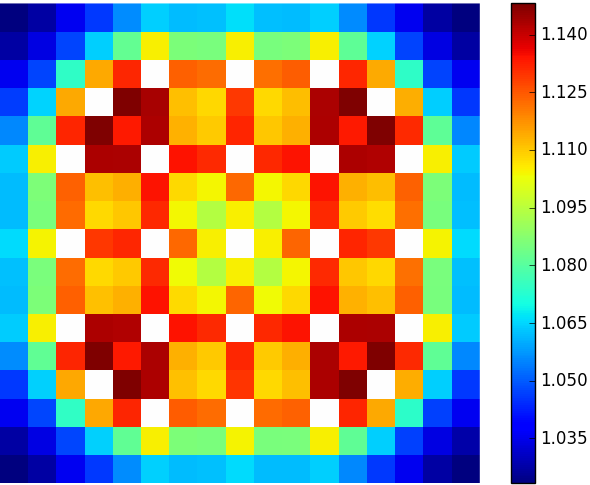
\includegraphics[width=\linewidth]{figures/assembly/fission-rates}
  \caption{}
  \label{fig:fiss-assm}
\end{subfigure}%
\begin{subfigure}{0.45\textwidth}
  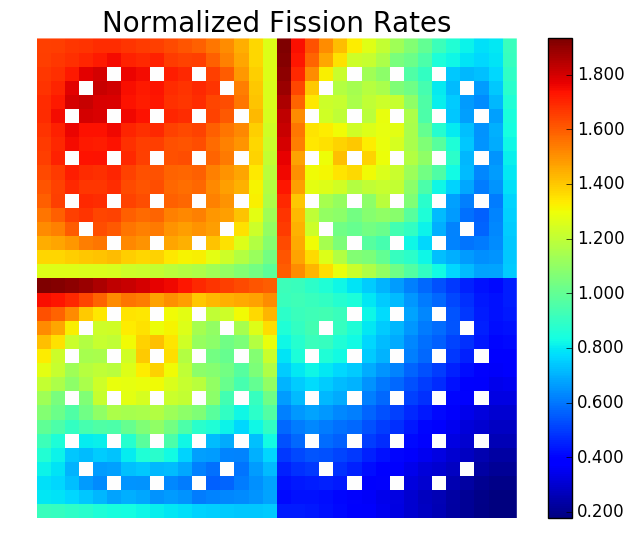
\includegraphics[width=\linewidth]{figures/colorset/fission-rates}
  \caption{}
  \label{fig:capt-assm}
\end{subfigure}
\caption{Reference OpenMC fission rates for the assembly (a) and colorset (b) benchmarks.}
\label{fig:benchmarks-fiss-rates}
\end{figure*}


%%%%%%%%%%%%%%%%%%%%%%%%%%%%%%%%%%%%%%%%%%%%%%%%%%%%%%%%%%%%
\subsection{MGXS Generation with OpenMC}
\label{subsec:openmc}

The \texttt{openmc.mgxs} module was employed to generate MGXS tallied CASMO's seventy energy group structure \cite{rhodes2006casmo}. Two OpenMC eigenvalue calculations were performed for the 1.6\% and 3.1\% enriched fuel pins, each in an infinite, repeating array\footnote{An infinite, repeating array of fuel pins is modeled by a single fuel pin with reflective boundary conditions.}, to generate MGXS for the fuel, zircaloy cladding, helium gap and borated water moderator. An additional OpenMC eigenvalue calculation of the entire geometry for benchmark was performed to generate MGXS for those pins without any fissile material -- namely, the CRGTs, BPs and instrument tubes. The seventy group MGXS were condensed to CASMO's 8- and 2-group structures using the \texttt{openmc.mgxs} module's data processing features.

Each OpenMC simulation included 100 inactive and 900 active batches of 10$^{6}$ particle histories per batch. The OpenMC simulations used the ``iso-in-lab'' feature to eliminate scattering source anisotropy as one possible cause of approximation error between OpenMC and OpenMOC, since OpenMOC uses an isotropic scattering source.


%%%%%%%%%%%%%%%%%%%%%%%%%%%%%%%%%%%%%%%%%%%%%%%%%%%%%%%%%%%%
\subsection{Multi-Group Calculations with OpenMOC}
\label{subsec:openmoc}

The MGXS generated by OpenMC were supplied to OpenMOC \cite{boyd2014openmoc} for deterministic multi-group transport calculations. The OpenMOC code solves the method of characteristics form of the neutron transport equation for 2D fixed source and eigenvalue calculations. OpenMOC approximates the scattering source as isotropic and the neutron source as constant across each spatial zone. The OpenMOC simulations used a characteristic track laydown with 128 azimuthal angles and 0.05 cm spacing. The root mean square of the energy-integrated fission source in each spatial zone was converged to 10$^{-5}$. The eigenvalues and pin-wise fission rates computed by OpenMOC are compared to the OpenMC reference solutions for both benchmarks in the following section.


%%%%%%%%%%%%%%%%%%%%%%%%%%%%%%%%%%%%%%%%%%%%%%%%%%%%%%%%%%%%%%%%%%%%%%%%%%%%%%%
\subsection{Results}
\label{subsec:results}
%%%%%%%%%%%%%%%%%%%%%%%%%%%%%%%%%%%%%%%%%%%%%%%%%%%%%%%%%%%%%%%%%%%%%%%%%%%%%%%

Both benchmarks were modeled with OpenMOC using MGXS generated by OpenMC using the single-step framework. The OpenMOC eigenvalues were compared to the reference OpenMC eigenvalues from \autoref{tab:keff-reference}. The eigenvalue bias $\Delta\rho$ was calculated by comparing the eigenvalue $k_{eff}^{MOC}$ from OpenMOC to the reference eigenvalue $k_{eff}^{MC}$ computed by OpenMC in units of per cent mille (pcm):

\begin{equation}
\label{eqn:delta-rho}
\Delta\rho = \left(k_{eff}^{MOC} - k_{eff}^{MC}\right) \times 10^{5}
\end{equation}

The bias is listed for both benchmarks in \autoref{tab:keff-bias}. It should be recalled that isotropic in lab scattering is used by OpenMC to compute both the reference solution and the MGXS. If anisotropic scattering were employed in OpenMC, one would expect quite different biases without a robust implementation of a higher order scattering kernel in OpenMOC.

\begin{table}[h!]
  \centering
  \caption{OpenMOC eigenvalue bias $\Delta\rho$.}
  \label{tab:keff-bias} 
  \begin{tabular}{l l r r r}
  \toprule
  \textbf{Benchmark} & \textbf{MGXS Scheme} & \textbf{2-Group} & \textbf{8-Group} & \textbf{70-Group} \\
  \midrule
  \multirow{2}{*}{Assembly} & Multi-Step    & -132 & -68 &   31 \\
                            & Single-Step &   60 & -72 & -161 \\
  \midrule
  \multirow{2}{*}{Colorset} & Multi-Step    & 2103 & 267 &   46 \\
                            & Single-Step & 1818 & 478 & -142 \\
  \bottomrule
\end{tabular}
\end{table}

The OpenMOC energy-integrated pin-wise fission rates were compared to the reference OpenMC fission rates \autoref{fig:benchmarks-fiss-rates}. The percent relative errors for each pin's fission rates were computed and the maximum and mean errors are listed in \autoref{tab:fiss-errors}, respectively. In particular, the maximum errors are the maximum of the absolute values of the errors along with the appropriate sign, while the mean errors are the averages of the absolute error magnitudes.

\begin{table}[h!]
  \centering
  \caption{OpenMOC max and mean fission rate percent relative errors.}
  \label{tab:fiss-errors}
  \begin{tabular}{l l c c c}
  \toprule
  \textbf{Benchmark} & \textbf{Metric} & \textbf{2-Group} & \textbf{8-Group} & \textbf{70-Group} \\
  \midrule
  \multirow{2}{*}{Assembly} & Max  & 2.387 & 0.643 & 0.375 \\
                            & Mean & 0.951 & 0.231 & 0.073 \\
  \midrule
  \multirow{2}{*}{Colorset} & Max  & 11.024 & 2.773 & 0.670 \\
                            & Mean & 4.964  & 1.029 & 0.147 \\
  \bottomrule
\end{tabular}
\end{table}

The spatial distributions of fission rate errors for the single-step framework are plotted as heatmaps for each benchmark in \autoref{fig:fiss-errors}. The heatmaps illustrate systematic trends in the pin-wise fission errors which correlate with spatial heterogeneities in each benchmark. In particular, the fission rates are generally underpredicted for pins adjacent to a single CRGT, but overpredicted for pins adjacent to two CRGTs in the assembly. In addition, the errors are largest for pins along the inter-assembly and assembly-reflector interfaces for the colorset benchmark.

%For the PWR benchmarks modeled here, the moderation provided by neighboring CRGTs and reflectors softens the flux for nearby fuel pins and should be modeled when collapsing pin-wise MGXS for high-fidelity multi-group transport calculations.

\begin{figure*}[h!]
\centering
\begin{subfigure}{0.45\textwidth}
  \centering
  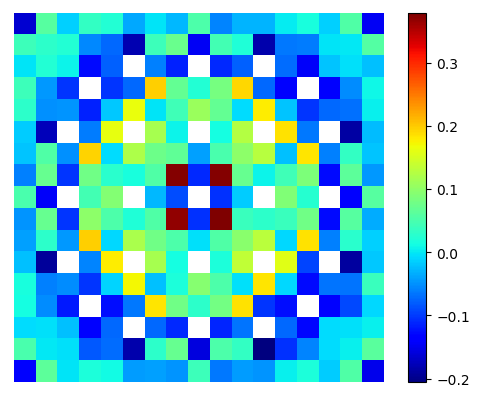
\includegraphics[width=\linewidth]{figures/assembly/fiss-single-step-errors}
  \caption{}
  \label{fig:assm-fiss-single-step-error}
\end{subfigure}%
\begin{subfigure}{0.45\textwidth}
  \centering
  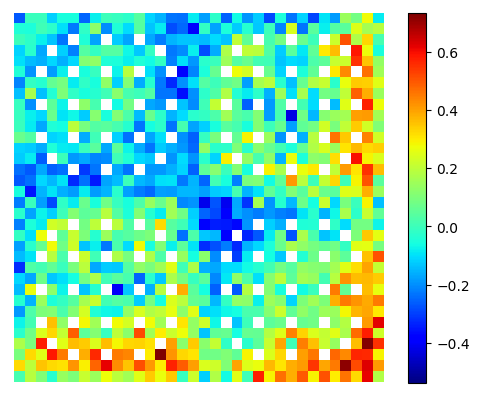
\includegraphics[width=\linewidth]{figures/colorset/fiss-single-step-errors}
  \caption{}
  \label{fig:colorset-fiss-single-step-error}
\end{subfigure}
\caption{OpenMOC fission rate percent relative errors for the assembly (a) and colorset (b) benchmarks.}
\label{fig:fiss-errors}
\end{figure*}
